\documentclass[a4paper,11pt]{article}
\usepackage[utf8]{inputenc}
\usepackage{apacite}
\usepackage[pdftex]{graphicx}
\providecommand{\keywords}[1]{\textbf{Palabras clave:} #1}
\begin{document}
	\title{Evaluación de cGAMP Ace-DEX MPs como adyuvante en la vacuna del virus de la influenza en ratones inmunosuprimidos}
	\author{Pablo Vargas Rodríguez, Alberto Priones Perez}
	\date{14 de Septiembre de 2020}
	\maketitle
	\begin{abstract}
El objetivo del proyecto será evaluar el efecto como adyuvante de las micropartículas de dextrano acetilado con cGAMP, un estimulador de genes interferón, en la vacuna de la gripe en sujetos inmunocomprometidos. En estudios previos ha sido revelado su gran papel en la estimulación equilibrada Th1/Th2, favoreciendo tanto la respuesta celular como la humoral. Debido a la falta de vacunas realmente eficaces en pacientes inmunocomprometidos, se va a evaluar el uso de este adyuvante en ratones inmunosuprimidos con prenidsona y cortisol.\\
Informacion adicional y acceso: https://github.com/pabloovar/proyecto\_final
\\ \\
\keywords{Ace-DEX, STING, inmunocomprimidos, vacunas, influenza, gripe, adyuvante, cGAMP}
	\end{abstract}

\section{Introducción}
Lejos de lo que pueda parecer, la capacidad de inducir una respuesta inmunitaria fuerte de una vacuna no está en el antígeno per se, no es necesariamente ese patógeno atenuado/inactivado el responsable del desarrollo de una inmunidad. En este baile, no solo participan el sistema inmunitario y el antígeno, sino que una parte importante de las vacunas son sus adyuvantes, dicho de otra forma, todo aquello que acompaña al antígeno con el objetivo de modular la respuesta inmune en una preparación vacunal.
\\En muchas ocasiones, el antígeno es incapaz de activar de forma eficaz al sistema inmunitario y son los adyuvantes los responsables directos del desarrollo de una inmunidad fuerte.
Numerosos son los esfuerzos que se están produciendo en el estudio de nuevos y mejorados adyuvantes, capaces de mejorar la forma en que las vacunas tradicionales activaba al sistema inmunitario.
\\Uno de los mencionados ejemplos de nuevos adyuvantes es el que presentamos en el título. Este se basa en el empleo de moléculas, como el cGAMP, capaces de activar a genes estimuladores de interferones (STING), transportadas dentro de micropartículas de dextrano acetilado (Ace-DEX MPs).\cite{Ady}

\subsection{Dextrano y genes STING}
Los polímeros de dextrano que se proponen emplear como medio de transporte de cGAMP, es una forma modificada del mismo polímero, aprobado por la FDA, el cual se ha modificado añadiendo grupos acetal cíclicos o metoxiacetal acíclicos.
\\El Ace-DEX es un compuesto biocompatible, biodegradable, de síntesis sencilla y estable a temperaturas elevadas. Además, se dirige específicamente a las células presentadoras de antígeno profesionales debido a su tamaño y, una vez fagocitadas, gracias a la sensibilidad ácida de estas micropartículas, el ambiente ácido del fagolisosoma provoca una rápida liberación del contenido de estas partículas.
\\Como decimos, cuando las micropartículas de Ace-DEX se introducen en un medio acuoso-ácido, se produce la hidrólisis de estos grupos acetal, convirtiendo al antes soluble en solventes orgánicos Ace-DEX, en el polímero soluble en agua que es el dextrano. Además, variando la forma en que estas partículas se sintetizan, podemos modificar la forma en que se liberan los contenidos de las micropartículas de dextrano, permitiendo que se libere su contenido en pocos minutos o que lo hagan durante meses.
\begin{figure}[h]
	\centering
	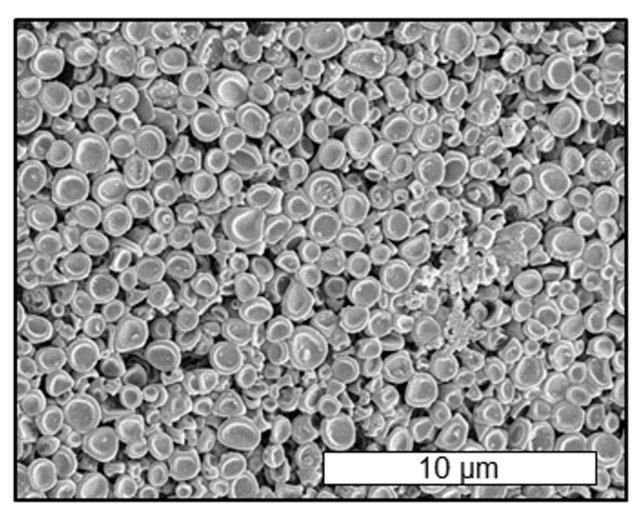
\includegraphics[scale=0.5]{Imágenes/dextrano}
	\caption{Microscopía electrónica de barrido de MP de dextrano}
	
	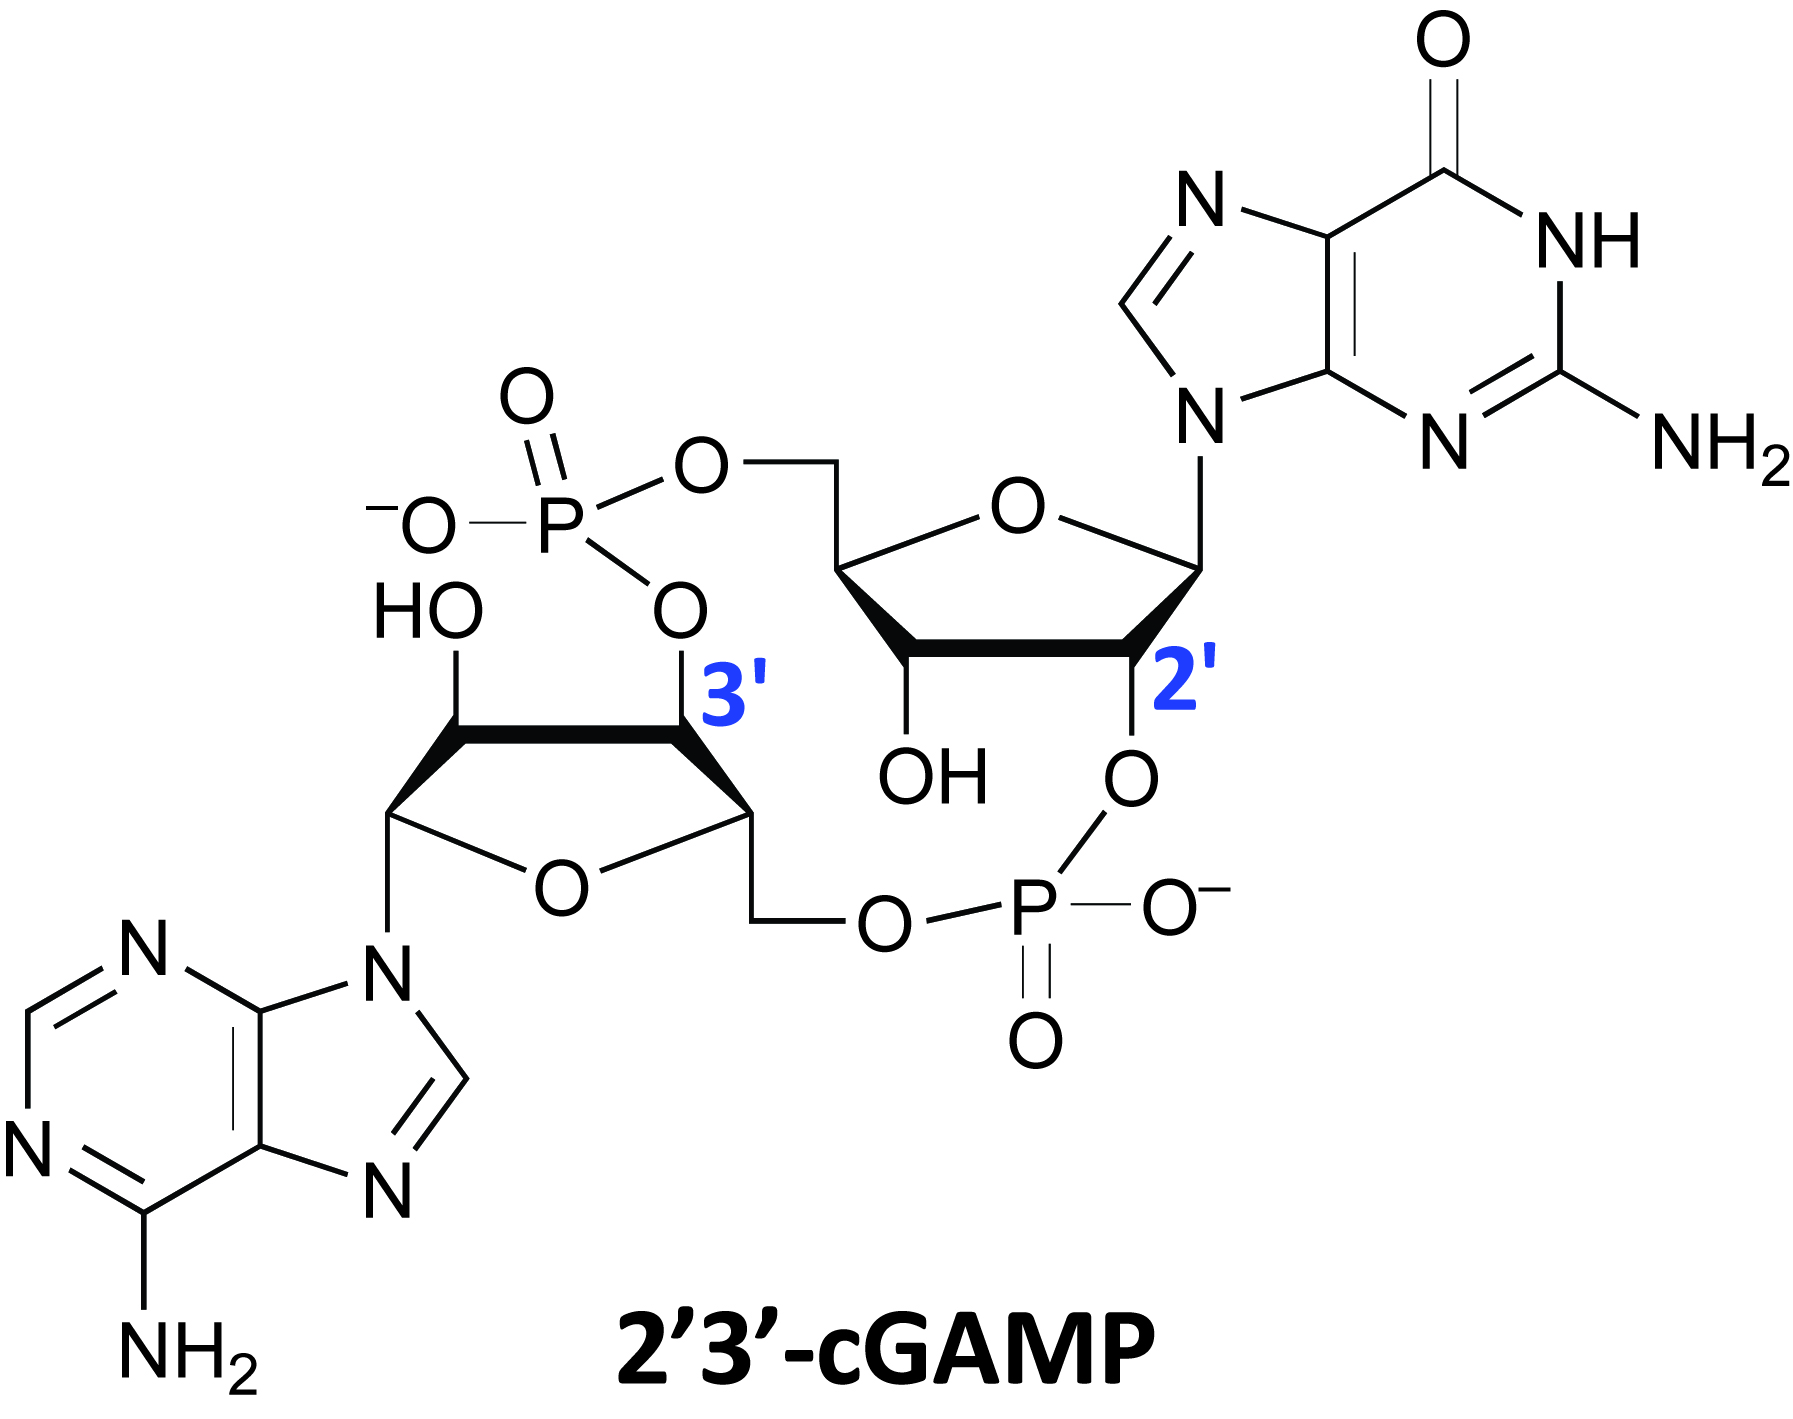
\includegraphics[scale=0.1]{Imágenes/GAMP}
	\caption{Estructura cGAMP}
\end{figure}
Estas micropartículas de dextrano son una forma ingeniosa y muy efectiva de conseguir una entrega intracelular y de liberación controlada de cualquier compuesto que se desee. 
\\En nuestro caso, analizaremos la posibilidad de emplear estas micropartículas para introducir en las células del sistema inmunitario un adyuvante capaz de activar a los genes STING.
\\Los genes STING (\textbf{STimulator of INterferon Genes}), son, como su nombre indica, genes relacionados con la síntesis de interferones, de tipo I concretamente. Lo que se propone emplear como activador de esta proteína son dinucleótidos cíclicos, como 3"3" cyclic GMP-AMP (cGAMP).
\\El principal problema de dirigir un tratamiento hacia esta diana es su localización celular, ya que esta proteína transmembrana se sitúa en la membrana del RE, de ahí el interés de usar las micropartículas de dextrano. En comparación, los dinucleótido cíclicos podrían administrarse de forma soluble, pero la respuesta administrados con las micropartículas propuestas aumenta su actividad es hasta 100 veces mayor.
\\Gracias a la investigación de Junkins et al. sabemos que el adyuvante propuesto es capaz de solventar el problema de las formulaciones vacunales basadas en subunidades proteicas y, a diferencia de los adyuvantes tradicionales, es capaz de inducir una respuesta potente y balanceada Th1/Th2. Esta respuesta es potenciada tanto a nivel humoral como celular consiguiendo una potente producción de INF-I y citoquinas pro-inflamatorias a nivel local, encontrando las MP únicamente en los nódulos linfáticos próximos al lugar de la infección (sin acumulación en otros órganos, indicando que no se produce una inflamación sistémica).
\\Su efecto fue probado junto con la proteína HA del virus de la gripe, consiguiendo resultados esperanzadores y una protección robusta a largo plazo. Consigue expandir el centro germinal de células B y las células T memoria.
\\Además, su producción mediante electrospray es escalable y eficiente y se la esterilización utilizando radiación gamma no afecta a su estructura, convirtiéndolo en un adyuvante idóneo.

\subsection{Vacuna de la Gripe}
Dadas las características del nuevo adyuvante que se propone, este podría ser empleado para mejorar la respuesta inmunitaria de vacunas comercializadas, cuya actividad, si bien suficiente, dista mucho de niveles óptimos, en cuanto a activación del sistema inmunitario y longevidad de la inmunidad.
\begin{figure}[h]
	\centering
	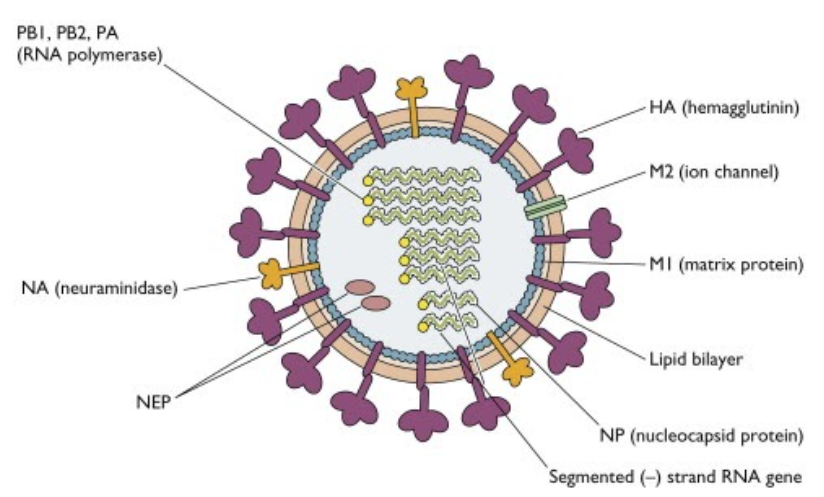
\includegraphics[scale=0.7]{Imágenes/influenza}
	\caption{Virus de la gripe}

\end{figure}
\\La vacuna de la gripe, como todos sabemos ya, tiene el principal inconveniente de que se necesitan nuevas formulaciones todos los años debido a la característica intrínseca de mutación del virus. Este es un problema, actualmente, difícil de combatir y nuevas estrategias de diseño de vacunas e identificación de antígenos son necesarias para poder solventar el problema.
\\Por otro lado, estas vacunas están preparadas con virus inactivados y fraccionados o a partir de antígenos de superficie virales, y este tipo de vacunas, en general, se caracterizan por no desarrollar una respuesta inmune completa, la activación de células T suele ser menor de lo deseable. De media, las vacunas de la gripe tienen una eficacia de entorno al 50\%  y la duración de los anticuerpos específicos producidos dura de 6 a 12 meses .
\\Si bien estos valores son suficientes como para prevenir y disminuir los casos e incidencia de la gripe, estos son valores muy mejorables. Es aquí, donde el empleo del adyuvante propuesto puede mejorar tanto la activación del sistema inmunitario y la eficacia de la vacuna como, por tanto, la duración de la inmunidad generada.
\\Otro ejemplo que pone en evidencia la eficacia y duración de la inmunidad adquirida a largo plazo es la vacuna del cólera. Esta vacuna está formada por el la bacteria causante de la enfermedad, inactivada, más la toxina B que esta produce. Al igual que antes, esta vacuna sufre problemas semejantes a la vacuna de la gripe. Inicialmente, esta vacuna ofrece unos porcentajes de protección frente a la bacteria Vibrio cholerae cercana al 100\% en algunos casos, pero esta baja más de un tercio en los primeros meses tras la aplicación y casi desaparece a los pocos años. Estos valores son adecuados para su uso como vacuna para viajeros a regiones en las que es endémica y para personas con riesgo continuado de infección se recomienda la revacunación tras 3 años.
\\Un experimento que podría proponerse para la determinación de la efectividad de esta vacuna, de forma que pudieran compararse sus efectos con las ya licenciadas, podría parecerse al siguiente:
Continuando con el ejemplo de la gripe, por ejemplo, nuestra vacuna podría basarse en las que actualmente se usan, virus inactivados, pero con la adición de estas partículas de dextrano y los activadores de los genes STING que portan. 
\\El experimento sería simple, visto que este adyuvante es seguro y eficaz en su uso en personas. Así, vacunaríamos a dos grupos de personas, susceptibles de contagiarse del virus, uno con la vacuna tradicional y el segundo con nuestra propuesta; el primero actuaría como control y nos permitiría comparar cómo evoluciona la segunda.
\\Así, buscaríamos que en el grupo de la vacuna experimental el porcentaje de incidencia de la gripe fuera menor que en el control, es decir, que el número de casos registrados de gripe fuera menor en el grupo de la vacuna experimental que en el de las vacunas licenciadas.
\\Más a largo plazo, buscaríamos medir los niveles de anticuerpos específicos contra el virus de la gripe, o más concretamente, poblaciones de células B plasmáticas productoras de los anticuerpos específicos.

\subsection{Vacunas en inmunocomprometidos}
Las personas inmunocomprometidas constituyen el grupo con más riesgo de mortalidad y morbilidad a causa de enfermedades evitables por vacunación. En general la vacunación de determinadas enfermedades como la gripe es recomendada, aunque debido a la heterogeneidad de las inmunodeficiencias su estudio se complica y los datos de eficacia son limitados. \cite{inmunodef} Además, en estos pacientes no se pueden utilizar vacunas vivas atenuadas por el riesgo de reversión. 
\\Un grupo de pacientes inmunocomprometidos bastante importante son los inmunosuprimidos por trasplantes de órganos sólidos. En estos la inmunogenicidad conseguida durante la vacunación es bastante pobre y la mejora de la respuesta por el uso de adyuvantes tradicionales no ha dado buenos resultados en el caso de la vacuna de la gripe. 
\\Se han realizado estudios del uso del adyuvante MF59 (esqualeno, polisorbato-80, trioleato de sorbitano en emulsión O/W)para la vacunación de la gripe en pacientes receptores de riñón pero la mejora de la respuesta no era significativa en general \cite{inmunodef2}:
Ratios de seroconversión vacunas con MF59 vs sin:
\begin{itemize}
	\item 71\% vs 55.2\% p=0.21
	\item 84.6\% vs 58.3\% p=0.039 (18-64 años de edad)
\end{itemize}
Datos no lo suficientemente significativos para aceptar la mejora de la respuesta. Sin embargo el objetivo principal de este estudio no era evaluar su efecto sino demostrar que los adyuvantes no ejercieran un efecto perjudicial en los pacientes.

Los datos de Ace-DEX cGAMP MP parecen indicar que es un muy buen adyuvante e idóneo para evaluar en estos pacientes inmunosuprimidos. Además, debido a que se ha demostrado que tiene un efecto local no debería suponer un riesgo para el órgano trasplantado. 

Otros grupos importantes de inmunocomprometidos son los receptores de células madres hematopoyéticas, pacientes tratados de cáncer o con enfermedades autoinmunes o inflamatorias. En trasplantes de células madre hematopoyéticas las vacunas son protectoras pero pobres, con bajos ratios de seroconversión (19-32\%) y niveles bajos de IgM. Estos también son grupos donde la evaluación del efecto de este adyuvante sería interesante.

\section{Materiales y Métodos}
\subsection{Síntesis de cGAMP Ace-DEX MP}
El método que se propone emplear para la síntesis de las micropartículas de dextrano, a la vez que se encapsulan los adyuvantes de dinucleótido cíclicos, está basado en una técnica de electrospray, o rociado electrohidrodinámico coaxial. Esta técnica tiene varias ventajas, como que se trata de un método de síntesis que puede trabajar en contínuo y que permite la síntesis y encapsulación en un único paso.
\\La base del proceso de síntesis es simple en concepto. La solución orgánica en la que se disuelve el dextrano y la solución acuosa que contiene el cGAMP se hacen pasar por una aguja especial, en la que la solución acuosa circula por el centro de la aguja y la solución orgánica por un conducto concéntrico exterior a esta. Así, se forma una cubierta de dextrano que engloba un núcleo acuoso.
\\Ambas soluciones fluyen a través de la aguja, dentro de sus conductos separados, de forma continua. El extremo de la aguja, por la que salen se encuentra altamente cargado, con un potencial eléctrico muy negativo, lo cual permite la evaporación de los solventes y formación de las micropartículas.
\\Finalmente, estas micropartículas cargadas se recogen sobre una placa metálica cargada con el signo opuesto, positivamente, de forma que se adhieren rápidamente a ella y pueden ser fácilmente recolectadas.
\\Después se determinaría la eficiencia de la encapsulación y la capacidad de carga de las MPs para comprobar que el proceso se lleva a cabo de manera correcta al comprobar los datos con la bibliografía. 
\\También se sintetizan MPs vacías, su interior únicamente contiene agua de pureza molecular, para ser usadas como control negativo.
\\El último paso en el proceso de síntesis de las micropartículas de Ace-DEX es determinar la eficiencia de encapsulación del cGAMP en las mismas.
\\Esto se hizo extrayendo el cGAMP de las micropartículas sintetizadas, empleando una disolución de diclorometano y agua, y posteriormente, midiendo la concentración mediante una cromatografía líquida y espectrofotometría.
\\Se determinaron dos parámetros clave para observar la eficiencia de la técnica, la capacidad de carga, cociente entre la masa del adyuvante y las MP, y la eficiencia de encapsulación, la masa de adyuvante encapsulada entre la masa máxima teórica.
\begin{displaymath}
	Capacidad de carga(\%) =  \frac{Masa cGAMP}{Masa MP} * 100
\end{displaymath}
\begin{displaymath}
	Eficiencia de Encapsulacion (\%) = \frac{Masa cGAMP}{Masa cGAMP Maxima  teorica} * 100
\end{displaymath}

\bibliographystyle{apacite}
\bibliography{biblioproyecto}

	
\end{document}